\documentclass[11pt,a4paper]{article}
\usepackage[margin=22mm]{geometry}
\usepackage[T1]{fontenc}
\usepackage{lmodern,amsmath,booktabs,array,xcolor,tikz}
\usepackage[hidelinks]{hyperref}
\setlength{\parindent}{0pt}
\setlength{\parskip}{6pt}
\newcommand{\question}[2]{\subsection*{Question #1 \hfill (#2\%)}}
\newcommand{\signal}[1]{\texttt{#1}}
\newcommand{\bus}[3]{%
  \draw (#2,#1)--({#2+.13},{#1+.17})--({#2+.87},{#1+.17})--({#2+1},#1)
    --({#2+.87},{#1-.17})--({#2+.13},{#1-.17})--cycle;
  \node[font=\scriptsize] at ({#2+.5},#1) {#3};}
\newcommand{\clockrow}[2]{%
  \node[anchor=east,font=\small] at (-.2,#1) {Clk};
  \foreach \i in {0,...,#2} {
    \draw (\i,#1)--(\i,{#1+.3})--({\i+.5},{#1+.3})--({\i+.5},#1)--({\i+1},#1);}}
\begin{document}
\setlength{\emergencystretch}{2em}
\begin{center}
{\Large\bfseries Digital System Design and Implementation}\\[5pt]
{\large Final Exam (111/05/31)}\\
Spring 2022
\end{center}
\textbf{Total points: 100 points}
\begin{itemize}
\item Please put all your modules in \textbf{one Verilog file} named by\\
\signal{DSDXXXXXXXXX.v} or \signal{DSXDXXXXXXXX.sv},\\
where X is your student ID,
for example, \signal{DSD105501001.v}.
\item Ensure your module and input as well as output ports having
\textbf{the same module/port names} as described in the following.
\item \textbf{Open Book!!!!}
\end{itemize}

In this final exam, we want to test one sequence with specific patterns.
Please write each module first.

\question{1}{10}
Please write a counter with asynchronous reset and positive edge trigger.
The counter will start to count from ``1'' to ``1023'' and back to ``1''
only when the ``En'' signal is high.
\begin{verbatim}
module EnCounter(CounterOut, Clk, Reset, En);
    ...
endmodule
\end{verbatim}
\textbf{Timing figure (redrawn).} The period of Clk is 100 ns. The labeled
CounterOut intervals below are the original sequence; the changes in En
occur between rising edges as drawn.
\begin{center}
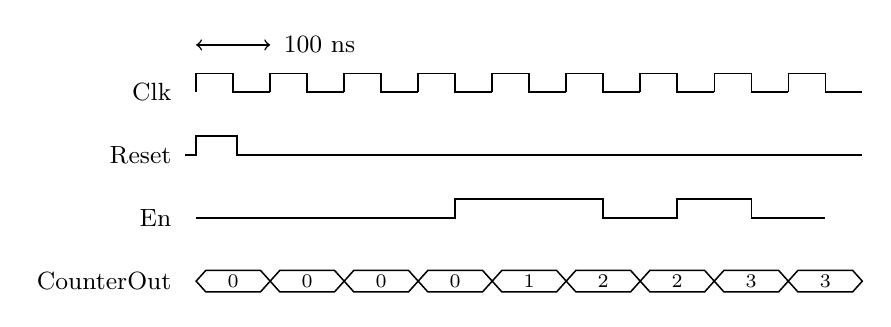
\begin{tikzpicture}[x=.94cm,y=.8cm,line width=.55pt]
\clockrow{3}{8}
\draw[<->] (0,3.75)--(1,3.75);
\node[font=\small,anchor=west] at (1.05,3.75) {100 ns};
\node[anchor=east,font=\small] at (-.2,2) {Reset};
\draw (-.15,2)--(0,2)--(0,2.3)--(.55,2.3)--(.55,2)--(9,2);
\node[anchor=east,font=\small] at (-.2,1) {En};
\draw (0,1)--(3.5,1)--(3.5,1.3)--(5.5,1.3)--(5.5,1)
  --(6.5,1)--(6.5,1.3)--(7.5,1.3)--(7.5,1)--(8.5,1);
\node[anchor=east,font=\small] at (-.2,0) {CounterOut};
\foreach \i/\v in {0/0,1/0,2/0,3/0,4/1,5/2,6/2,7/3,8/3} {\bus{0}{\i}{\v}}
\end{tikzpicture}
\end{center}

\question{2}{10}
Please write a module called ``Rotator'' that will rotate the 4-bit input
``RIn'' to the left by $r$ bits, where $r=0,1,2,3$, and is set by 2-bit
input signal ``Rb''. The output is called ``ROut''.
\begin{verbatim}
module Rotator(Rout, RIn, Rb);
    ...
endmodule
\end{verbatim}

\question{3}{10}
Please write a synchronous read/write register file that has 8 words and
each word has 10 bits wide. The write enable signal ``WE'' is active high.
\begin{verbatim}
module RegisterFile(Q, D, Clk, WE, Add);
    ...
endmodule
\end{verbatim}

\question{4}{15}
Please write a module called ``PatternCheck'' that will generate ``1'' at
exactly the same clock time when 4-bit input pattern is matched with a
pre-defined 4-bit pattern specified by the user using ``Load'' signal.
The input pattern is sent by ``InPattern'' indicated by ``ValidIn'' signal
that will be activated only after loading operation of the user pattern
as shown in the following, where $0\leq p\leq15$.
(You don't need to write test pattern.)
\begin{verbatim}
module PatternCheck(Judge, InPattern, ValidIn,
                    UserPattern, Load, Clk, Reset);
    ...
endmodule
\end{verbatim}
\textbf{Block figure (editable signal table).}
\begin{center}
\begin{tabular}{lll}\toprule
Signal & Connection & Width shown in figure\\\midrule
ValidIn & Input to Pattern Check & 1\\
InPattern & Input to Pattern Check & 4\\
UserPattern & Input to Pattern Check & 4\\
Load & Input to Pattern Check & 1\\
Clk, Reset & Inputs to Pattern Check & ---\\
Judge & Output from Pattern Check & 1\\\bottomrule
\end{tabular}
\end{center}
\textbf{Timing figure (redrawn).} ``p'' remains symbolic as in the source;
it is not replaced with a particular test value. Judge is high in the
same input interval as the matching p, rather than the next interval.
\begin{center}
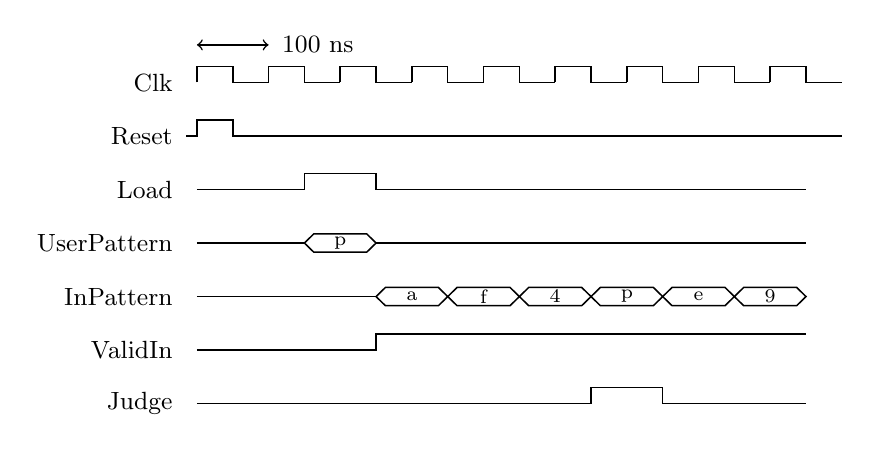
\begin{tikzpicture}[x=.91cm,y=.68cm,line width=.55pt]
\clockrow{6}{8}
\draw[<->] (0,6.7)--(1,6.7);
\node[font=\small,anchor=west] at (1.05,6.7) {100 ns};
\node[anchor=east,font=\small] at (-.2,5) {Reset};
\draw (-.15,5)--(0,5)--(0,5.3)--(.5,5.3)--(.5,5)--(9,5);
\node[anchor=east,font=\small] at (-.2,4) {Load};
\draw (0,4)--(1.5,4)--(1.5,4.3)--(2.5,4.3)--(2.5,4)--(8.5,4);
\node[anchor=east,font=\small] at (-.2,3) {UserPattern};
\draw (0,3)--(1.5,3);\bus{3}{1.5}{p}\draw (2.5,3)--(8.5,3);
\node[anchor=east,font=\small] at (-.2,2) {InPattern};
\draw (0,2)--(2.5,2);
\foreach \i/\v in {2.5/a,3.5/f,4.5/4,5.5/p,6.5/e,7.5/9} {\bus{2}{\i}{\v}}
\node[anchor=east,font=\small] at (-.2,1) {ValidIn};
\draw (0,1)--(2.5,1)--(2.5,1.3)--(8.5,1.3);
\node[anchor=east,font=\small] at (-.2,0) {Judge};
\draw (0,0)--(5.5,0)--(5.5,.3)--(6.5,.3)--(6.5,0)--(8.5,0);
\end{tikzpicture}
\end{center}

\question{5}{15}
Please write a module called ``MaskPatternCheck'' that will generate ``1''
at exactly the same time when some bits of the 4-bit input pattern are
matched with a pre-defined pattern specified by the user using ``Load''
signal. For example, we can specify pattern to be compared as
``\signal{4'b10?1}''. It means that the mask is ``\signal{4'b1101}'' and
we don't care the state of the third bit. If the input pattern is
``\signal{4'b1001}'' or ``\signal{4'b1011}'', the output flag ``Match''
will become ``1''. (You can reuse your codes of Q4.)
\begin{verbatim}
module MaskPatternCheck(Match, InPattern, ValidIn, Mask,
                        UserPattern, Load, Clk, Reset);
    ...
endmodule
\end{verbatim}
\textbf{Block figure (editable signal table).}
\begin{center}
\begin{tabular}{lll}\toprule
Signal & Connection & Width shown in figure\\\midrule
ValidIn & Input to Pattern Check with Mask & 1\\
InPattern & Input to Pattern Check with Mask & 4\\
UserPattern & Input to Pattern Check with Mask & 4\\
Load & Input to Pattern Check with Mask & 1\\
Mask & Input to Pattern Check with Mask & 4\\
Clk, Reset & Inputs to Pattern Check with Mask & ---\\
Match & Output from Pattern Check with Mask & 1\\\bottomrule
\end{tabular}
\end{center}
\textbf{Timing figure (redrawn).}
\begin{center}
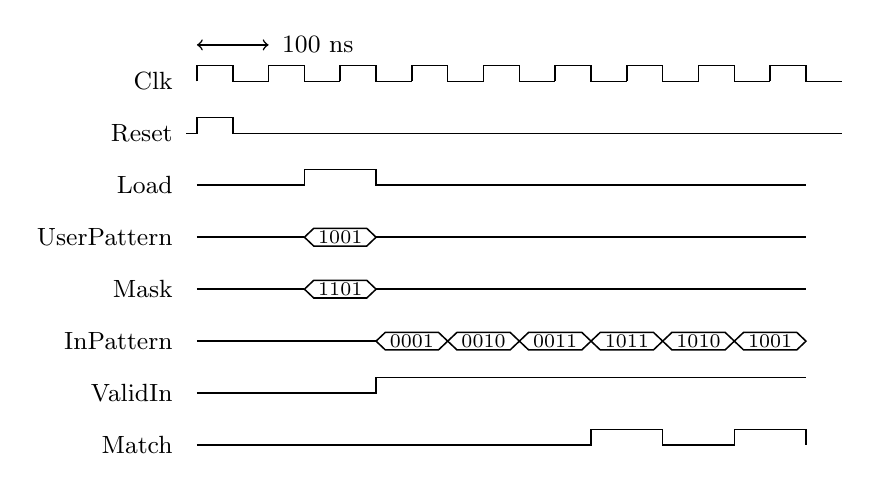
\begin{tikzpicture}[x=.91cm,y=.66cm,line width=.55pt]
\clockrow{7}{8}
\draw[<->] (0,7.7)--(1,7.7);
\node[font=\small,anchor=west] at (1.05,7.7) {100 ns};
\node[anchor=east,font=\small] at (-.2,6) {Reset};
\draw (-.15,6)--(0,6)--(0,6.3)--(.5,6.3)--(.5,6)--(9,6);
\node[anchor=east,font=\small] at (-.2,5) {Load};
\draw (0,5)--(1.5,5)--(1.5,5.3)--(2.5,5.3)--(2.5,5)--(8.5,5);
\node[anchor=east,font=\small] at (-.2,4) {UserPattern};
\draw (0,4)--(1.5,4);\bus{4}{1.5}{1001}\draw (2.5,4)--(8.5,4);
\node[anchor=east,font=\small] at (-.2,3) {Mask};
\draw (0,3)--(1.5,3);\bus{3}{1.5}{1101}\draw (2.5,3)--(8.5,3);
\node[anchor=east,font=\small] at (-.2,2) {InPattern};
\draw (0,2)--(2.5,2);
\foreach \i/\v in {2.5/0001,3.5/0010,4.5/0011,5.5/1011,6.5/1010,7.5/1001} {\bus{2}{\i}{\v}}
\node[anchor=east,font=\small] at (-.2,1) {ValidIn};
\draw (0,1)--(2.5,1)--(2.5,1.3)--(8.5,1.3);
\node[anchor=east,font=\small] at (-.2,0) {Match};
\draw (0,0)--(5.5,0)--(5.5,.3)--(6.5,.3)--(6.5,0)
  --(7.5,0)--(7.5,.3)--(8.5,.3)--(8.5,0);
\end{tikzpicture}
\end{center}

\question{6}{20}
Now, a 4-bit sequence with sequence length smaller than 1023 is going to
be processed. We need to check how many times the user pre-defined pattern
occurs and save the result in the address 4 of register file. If
``ValidIn''=0, the associated ``InPattern'' is invalid and it is not
counted in. Please use the template in the following and
\textbf{name the register file as U1} as described in the following.
(In addition to Register file, you can use previous modules freely.)
\begin{verbatim}
module PatternCount((InPattern, ValidIn, UserPattern,
                     Load, Clk, Reset);
    ...
    RegisterFile U1(.Q(), .D(), .Clk(), .WE(), .Add());
endmodule
\end{verbatim}

\question{7}{20}
Now, a 4-bit sequence with sequence length smaller than 1023 is going to
be processed. We need to check the positions of the pattern ``1?01'' with
mask ``1011'' occurs and save the position result of the last occurrence
of that pattern in the address 7 of register file. The starting position
index 1 corresponds the first data indicated by ``ValidIn''. If
``ValidIn''=0, the associated ``InPattern'' is invalid and its position
will not be saved. Please use the template in the following and
\textbf{name the register file as U1} as described in the following.
(In addition to Register file, you can use previous modules freely.)
\begin{verbatim}
module PatternPosition((InPattern, ValidIn, Clk, Reset);
    ...
    RegisterFile U1(.Q(), .D(), .Clk(), .WE(), .Add());
endmodule
\end{verbatim}

\bigskip\hrule\smallskip
\textbf{Transcription and provenance note.} This editable LaTeX
transcription was checked against all three pages of
\signal{Final-Exam-2022.pdf}, supplied with this task. The exam instructions
above are historical source content. Figures have been redrawn in TikZ or
transcribed into tables; they are not solution code. Module names and port
order follow the printed PDF. Printed discrepancies are retained:
the SystemVerilog filename is printed as \signal{DSXDXXXXXXXX.sv};
Q2 prose says \signal{ROut} but its module header says \signal{Rout};
Q6 and Q7 headers each contain an extra opening parenthesis. Ellipses and
line wrapping have been normalized, without changing requirements. No
unprinted register-file collision rule, initialization rule, or invalid
data position-counting rule has been added to the original questions.
\end{document}
